\documentclass[tikz,border=10pt]{standalone}
\usepackage{amsmath}
\begin{document}
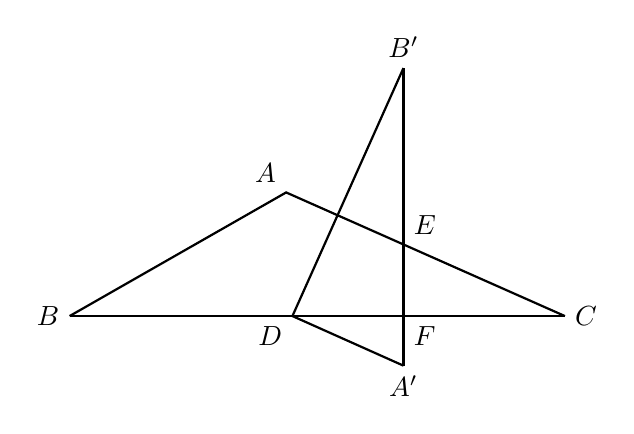
\begin{tikzpicture}[scale=1, line width=0.8pt]
  \coordinate (B) at (0,0);
  \coordinate (D) at (2.83,0);
  \coordinate (C) at (6.29,0);
  \coordinate (A) at (2.75,1.57);
  \coordinate (Bp) at (4.24,3.15);
  \coordinate (Ap) at (4.24,-0.63);
  \coordinate (E) at (4.24,0.91);
  \coordinate (F) at (4.24,0);

  \draw (B) -- (A) -- (C);
  \draw (B) -- (C);
  \draw (Bp) -- (D) -- (Ap);
  \draw (Bp) -- (Ap);

  \node[above left] at (A) {$A$};
  \node[left] at (B) {$B$};
  \node[right] at (C) {$C$};
  \node[below left] at (D) {$D$};
  \node[above] at (Bp) {$B'$};
  \node[below] at (Ap) {$A'$};
  \node[above right] at (E) {$E$};
  \node[below right] at (F) {$F$};
\end{tikzpicture}
\end{document}
